

\fancypagestyle{miEstilo504}{
   \lhead{5.4 Descripción de la aplicación}
   \rhead{Página \thepage}
   \lfoot{}
   \cfoot{}
   \rfoot{}
}

\pagestyle{miEstilo504}


\subsection{Medidas de seguridad}

Cuando hablamos de un sistema de videovigilancia hay que tener claro que la información grabada por la cámara es de carácter sensible, ya que puede invadir la privacidad de un conjunto de personas, y por lo tanto, hay que controlar quién tiene acceso a dicha información y qué mecanismos se utilizan para que cualquier persona no autorizada no pueda acceder a dicha información.

Además, dado que esta implementación hace uso de un bot de telegram, y dicho bot puede ser de carácter público, hay que tener incluso más cuidado, ya que no se quiere que ningún desconocido pueda tener control sobre nuestro sistema de seguridad que está vigilando nuestro entorno. Por ello, se ha provisto a la aplicación de unos mecanismos de identificación y autenticación simples pero efectivos.

\textbf{Primera medida de seguridad: API token}

En primer lugar, cuando el usuario crea el bot a través del \texttt{BotFather} \cite{ref31}, además de añadir un nombre, descripción \ldots al bot, se le proporciona un \texttt{API token} que consta de una serie de caracteres alfanuméricos, y que debe de ser almacenado como una contraseña. Dicho \texttt{API token} es necesario utilizarlo para configurar el servicio de bot de telegram más adelante. 


\begin{figure}[h]
	\centering
	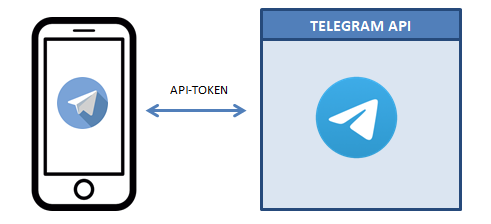
\includegraphics[scale=0.35]{images/36}
	\caption{Primera medida de seguridad}
	\label{img:seg1}
\end{figure}

Esta es la medida que nos aporta la aplicación de telegram para controlar el usuario que pueda administrar dicho bot.

El \texttt{API token} no permite la gestión del bot, pero por ahora si está permitido poder utilizar dicho bot y acceder a su conjunto de funcionalidades, por lo que esto sería un potencial riesgo.

Para prevenir este posible riesgo se ha implementado una segunda medida.

\textbf{Segunda medida: Lista blanca de usuarios}

Esta medida se basa en la implementación de una lista blanca que contiene los identificadores únicos de los usuarios que tienen permiso para utilizar el bot. Esta lista blanca está ubicada en el servicio del bot de telegram, y almacena los identificadores y nombres de usuario permitidos.

\begin{figure}[h]
	\centering
	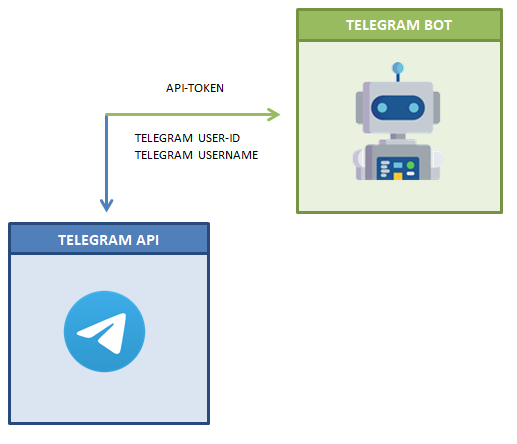
\includegraphics[scale=0.5]{images/37}
	\caption{Segunda medida de seguridad: Lista blanca de usuarios}
	\label{img:seg2}
\end{figure}

Con esta segunda medida, podemos permitir a los usuarios que queramos que tengan acceso a dicha información. Un ejemplo de esta lista blanca es el siguiente:

\vspace{-0.5cm}

\begin{verbatim}
  allowed_users = {
  				    'users':
		                 [
		                   {'id': telegram_user_id, 'username': telegram_username}, 
		                   {'id': bot_user_id, 'username': bot_username}
		                 ]
	              }
\end{verbatim}

\vspace{-0.5cm}


Si un usuario no permitido accede al bot e intenta utilizarlo se le mostrará el siguiente mensaje:

\vspace{-0.5cm}

\begin{verbatim}
You have not permission to access to this content
\end{verbatim}

\vspace{-0.5cm}

También, es importante destacar, que la \textbf{información} que viaja desde que el usuario accede a telegram, hasta que llega al servicio del bot de telegram \textbf{va cifrada}.

Las medidas aplicadas anteriormente sirven para controlar el acceso por parte de la aplicación de telegram, pero ¿y si alguna aplicación externa no autorizada intenta acceder a la \texttt{API} principal?

\texttt{Tercera medida: Autenticación usuario-contraseña}

El tercer mecanismo se basa en restringir el acceso a la \texttt{API} principal de la aplicación a través de una autenticación mediante usuario y contraseña. Esta autenticación la proporciona el módulo \texttt{authentication}, y se basa en comprobar si las credenciales de acceso son correctas,y por lo tanto, la \texttt{API} responderán a las peticiones recibidas.

Estas credenciales de acceso son necesarias para todos los servicios que quieran interactuar con la API, por lo tanto, deben de ser especificadas en el archivo de configuración \texttt{ 	authentication.yml} como se muestra a continuación:

\vspace{-0.5cm}

\begin{verbatim}
---

authentication:
    user: user
    password: sha256$tazHE31s$b4b54292237636e798e407dc935651f9af64a

\end{verbatim}

\vspace{-1cm}

Nótese que la contraseña está cifrada utilizando el algoritmo \texttt{sha256}. Para poder generar este hash, se ha proporcionado un script llamado \texttt{generate\_hash\_password.py} (ubicado en el directorio tools) para poder introducir la contraseña deseada, y se nos devuelve el hash de la contraseña.

En la siguiente figura, podemos observar como todos los servicios interaccionan con la \texttt{API} mediante un usuario y contraseña (menos con los módulos que los importa directamente).

\newpage

\begin{figure}[h]
	\centering
	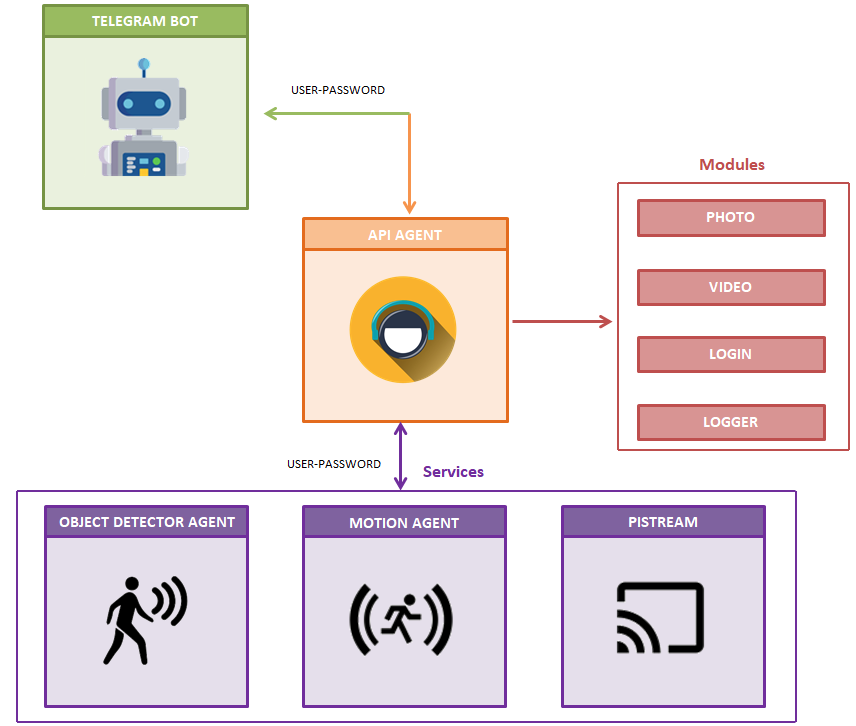
\includegraphics[scale=0.5]{images/38}
	\caption{Tercera medida de seguridad: Usuario y contraseña}
	\label{img:seg3}
\end{figure}
